\begin{figure}[t]
\centering
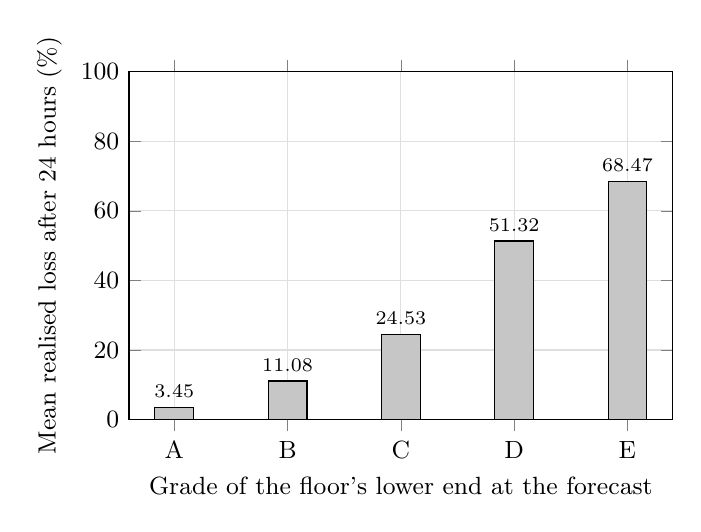
\begin{tikzpicture}
\begin{axis}[ybar, width=0.7\linewidth, height=6cm, bar width=14pt, symbolic x coords={A,B,C,D,E}, xtick=data, xlabel={Grade of the floor's lower end at the forecast}, ylabel={Mean realised loss after 24 hours (\%)}, ymin=0, ymax=100, grid=major, grid style={gray!25}, nodes near coords, nodes near coords style={font=\scriptsize}, tick label style={font=\small}, label style={font=\small}]
\addplot[fill=gray!45] coordinates {(A,3.4511) (B,11.0818) (C,24.5258) (D,51.3220) (E,68.4703)};
\end{axis}
\end{tikzpicture}
\caption{Mean loss of the 100 USDC reference position 24 hours after the forecast, by grade, over rated retrospective records (H4). Records per grade: A: 474; B: 127; C: 80; D: 84; E: 111. Computed by analysis/results.py from the released dataset.}
\label{fig:grades}
\end{figure}
